Chegou o dia da Maratona Mineira e a organização já tem as cores definidas para quase todos os problemas, faltando apenas um!
Para facilitar a visualização do placar e do ambiente de prova, diminuindo a chance de confusões com balões de cores muito similares,
a organização resolveu escolher esta última cor de forma que ela seja tão diferente das outras já selecionadas. As cores são codificadas
no sistema RGB, através de triplas de inteiros que representam as quantidades de vermelho, verde e azul, respectivamente,
na codificação da cor.

\begin{figure}[H]
    \centering
    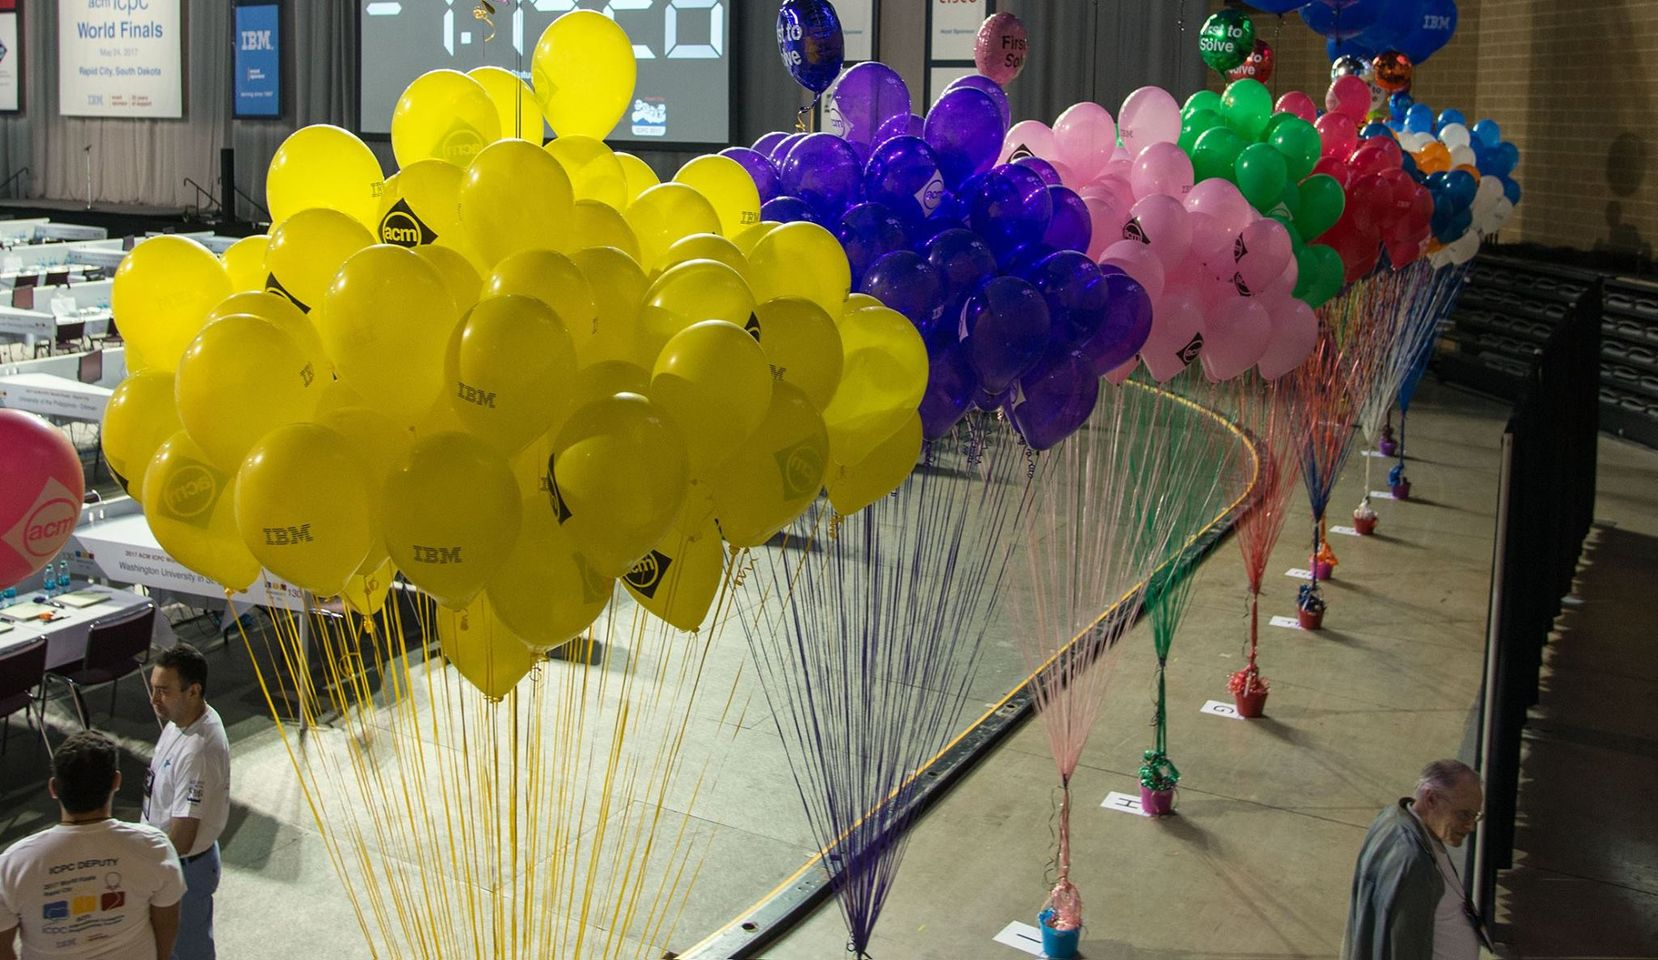
\includegraphics[width=8cm]{\CWD/baloes.jpg}
\end{figure}

Dadas duas cores, $(r_1,g_1,b_1)$ e $(r_2,g_2,b_2)$, calculamos a distancia entre elas como $d = |r_1-r_2| + |g_1-g_2| + |b_1-b_2|$.
Sua tarefa é encontrar qual seria a \textbf{cor que maximiza a menor distância daquelas já existentes}. Caso mais de uma solução exista,
aquela que minimiza a primeira coordenada da codificação deve ser escolhida. Persistindo o empate, deve ser escolhida aquela que minimiza
a segunda coordenada. Caso mais de uma solução ainda exista aplicando estes critérios, deve ser escolhida aquela que minimiza a terceira coordenada. Em outras palavras, queremos a menor solução de forma lexicográfica.

\section*{Entrada}

A primeira linha da entrada contém um inteiro $1 \leq N \leq 20$. Em seguida são dadas $N$ linhas, de forma que a $i$-ésima linha, contém 3 números
entre 0 e 255 (inclusivo), correspondendo ao código RGB da $i$-ésima cor já selecionada.

\section*{Saída}

A saída contém três inteiros $R, G, B$, que correspondem ao código da cor que maximiza a distância para as demais cores.

\section*{Restrições}

\begin{itemize}
\item $1 \leq N \leq 20$
\item $0 \leq R, G, B \leq 255$.
\end{itemize}


\section*{Exemplos}

\sampleio
